

\chapter{Fungují opatření? Korelace versus kauzalita} \label{Co_na_cem_zavisi}

\textit{Martin Šmíd, Aleš Kuběna}
\vspace{15mm}

\noindent Vzhledem k~tomu, do jaké míry se současná pandemie dotýká života většiny lidí, vzbudila nejen nebývalou vlnu zájmu vědecké komunity, ale ve značné míře i kontroverze v~tom, co o~ní vědci tvrdí. Již léta lze pozorovat podobnou kontroverzi týkající se příčiny klimatických změn, z~minulosti připomeňme např. spory o~škodlivosti kouření. Nyní tedy do této „války“ přibyla „bitva o~covid“. S~trochou nadsázky lze tvrdit, že se všechny tyto spory redukují na otázku, zda v~případě, že se dva jevy vyskytují současně (korelace), jeden z~nich způsobuje ten druhý (kauzalita).

Za všemi uvedenými kontroverzemi lze tušit společnou příčinu: neochotu změnit chování, které je v~podezření, že způsobuje (stávající či budoucí) problémy. V~případě sporů o~kouření je to neochota kuřáků upřít si své „potěšení“, tabákových firem vzdát se zisků a státu vzdát se spotřebních daní. U~sporů o~klima je to nechuť k~udržitelnému hospodaření v~protikladu k~zadlužování se na úkor budoucích generací. V~případě sporů o~covid-19 je to odpor k~nepopulárním omezujícím protiepidemickým
opatřením. Zmíněné kontroverze mají jistě i další důvody, například neochotu si daný problém vůbec připustit nebo neuchopitelnost problémů pro neodborníky -- dopátrat se nějaké hlavní příčiny lze stěží, obtížnost důkazů kauzality je ostatně tématem tohoto článku. Nicméně ať už je způsobilo cokoli, jsou tyto kontroverze realitou a je třeba se k~nim nějakým způsobem postavit.

\begin{figure}
\begin{center}
\begin{tabular}{cc}
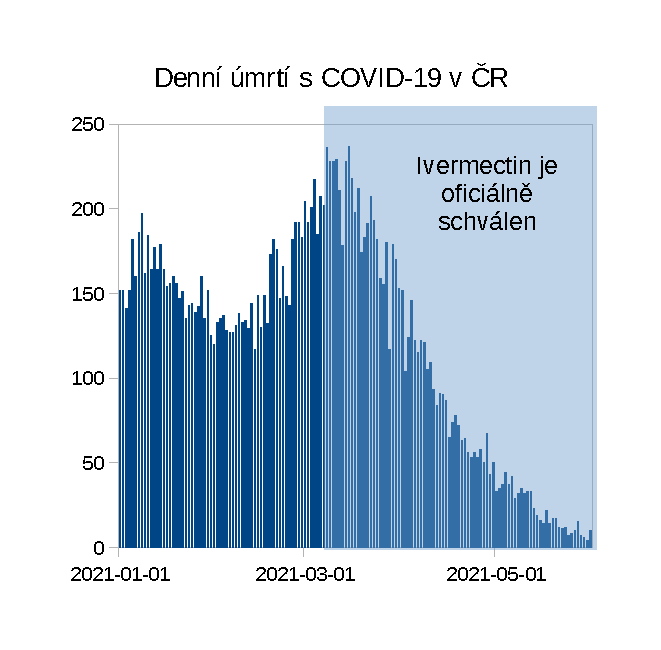
\includegraphics[width=0.4\textwidth]{pic/ivernectin.pdf} & 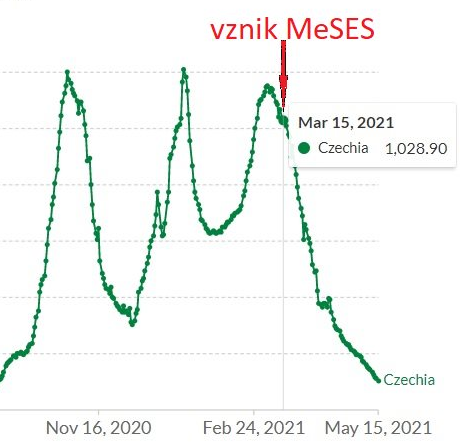
\includegraphics[width=0.4\textwidth]{pic/meses.png}\tabularnewline
\tabularnewline
\end{tabular}
\caption{Zdroj Qanon.cz, Twitter (vlevo), Petr Jedlička, Facebook (vpravo).}
\label{fig:iverjedl}
\end{center}
\end{figure}

Podstatu sporů o~covid dobře ilustruje obrázek \ref{fig:iverjedl}. Oba grafy, nalezené na sociálních sítích, nepochybně zobrazují tvrdá data -- první počty úmrtí a období,
kdy byl k~léčení covid-19 schválen kontroverzní
lék Ivermectin, jehož účinnost dosud nebyla prokázána \cite{mzcriver},
druhý přírůstky nových případů a období oficiální existence Mezioborové
skupiny pro epidemické situace \cite{zalozenimeses} známé pro svůj
striktně vědecký přístup a opatrnost při uvolňování restriktivních
opatření. Oba grafy působí sugestivně, oba naznačují příčinu poklesu případů
na jaře 2021, každý však ale diametrálně odlišnou. Ve skutečnosti však demonstrují pouze časovou souvislost, nikoli příčinnost -- kauzalitu. Přitom právě otázka kauzality je zde klíčová. Co bylo skutečnou příčinou jarního poklesu? I~v~jiných sporných otázkách se diskuse točí okolo kauzality. Je tím, co
způsobuje smrt, skutečně virus, nebo spíše jiné nemoci, na které by dotyční lidé stejně zemřeli? Byl to skutečně lockdown, co snížilo nárůst případů,
nebo by snížení díky jakési vnitřní dynamice epidemie nastalo i bez něj? Jakkoli
absurdně může poslední otázka znít, existuje nemalé množství publikací
snažících se dokázat druhou možnost. Za vlajkovou publikaci lze považovat \cite{bendavid2021assessing}
(pro diskusi o~této práci viz \cite{kluveitIoan}), z~domácích autorů
se v~tomto proudu angažují například \cite{hradsky2021demographic}. 

Patrně to mnohé překvapí, ale otázka kauzality je filozofická a věda na ni nikdy nedokáže definitivně odpovědět. V~principu je vždy možné, že vše, co zažíváme, je jen jakási sofistikovaná
virtuální realita, ve které všechno včetně výsledků vědeckých experimentů
někdo dopředu naprogramoval. Nakonec je vždy na člověku, zda argumenty
pro tvrzení, že jeden jev způsobuje druhý, vezme za své. Náš příspěvek
si klade za cíl prodiskutovat otázku kauzality hlouběji a vztáhnout
tuto diskusi na účinnost
protiepidemických opatření. Podotýkáme, že naším cílem není problematiku
zcela vyčerpat, případně podat jakési definitivní odpovědi. Spíše se snažíme
naznačit, jakým směrem by se dále mohla ubírat diskuse o~tom, co je
a co není vědecky podloženo.

\section*{Korelace a kauzalita}

Pokud jeden jev způsobuje druhý, projeví se to jejich korelací. Obráceně to však neplatí. Jak schválení léku Ivermectin, tak vznik MeSES jsou s~poklesem epidemie korelované, nedokazuje to však, že jej způsobily. Poučka {\em korelace neimplikuje kauzalitu (correlation does not imply causation)} patří k~základům kritického myšlení, často však bývá používána pro zpochybnění jakýchkoli nehodících se vědeckých výsledků. Často se pak stává, že diskuse nikam nevede, protože každá strana za kauzální uznává jen „své“ korelace, zatímco ty oponentovy zpochybňuje.

Jak z~tohoto bludiště ven? Podle \cite{shipley_2000} až na několik málo výjimek za každou korelací nějaká, možná neznámá, kauzální struktura stojí. Smyslem výše uvedené poučky je varovat před pokušením při korelaci $A$ a $B$ na místo oné struktury rovnou dosadit tu nejjednodušší $A\rightarrow B$ (šipka značí kauzalitu), případně jen vybírat z~množiny $A\rightarrow B, B\rightarrow A$. Na druhou stranu bychom se v~této potenciální složitosti neměli ztratit a následně na hledání kauzality rezignovat. Podle \cite{shipley_2000} i \cite{pearl2009causality} bychom se místo hledání „dokonalého“ kauzálního modelu měli raději pokusit navrhnout větší množství axiomatických modelů kauzálních vztahů spolu s~konkrétní datovou a modelovací podporou a pak vybrat ten nejlepší z~nich. Pravidla volby přitom mohou sledovat různé cíle, pro nás je v~případě šířeni viru SARS-CoV-2 důležité volit mezi následujícími dvěma:
\begin{itemize}
\item identifikovat kauzální řetězce v~epidemii nahlížené jako přírodní jev,
\item identifikovat ty z~příčin, které v~praxi dokážeme ovlivnit, a pokud možno kvantifikovat dopad případných intervencí.
\end{itemize}

Mnoho sporů týkajících se vědeckého uchopení současné pandemie spočívá v~tom, že každá strana upřednostňuje jeden z~výše uvedených pohledů a druhý považuje z~principu za nesprávný. Přitom se tyto pohledy nevylučují, pouze se každý zaměřuje na jinou stránku komplexního jevu -- pandemie. 

%Pokud se zaměříme na druhou možnost, evidentní kandidátkou na hledanou příčinu je frekvence rizikových kontaktů mezi lidmi, a tím i nefarmaceutická opatření, která tuto frekvenci snižují. Jakkoli je s podivem, že tento téměř evidentní fakt někdo zpochybňuje či marginalizuje, děje se to. Proto se této otázce věnujme podrobněji.

\subsection*{Hillova kritéria}

Způsobů, jak se pokoušet identifikovat kauzalitu, je více,
my zde uvádíme sadu kritérií navrženou v~roce 1965 Austinem Bradfordem Hillem
speciálně pro oblast epidemiologie \cite{hill1965environment}. Tato kritéria demonstrujeme na příkladu kauzálního vztahu protiepidemických opatření a velikosti epidemie. Konkretně zkoumáme několik souvisejících kandidátů na příčiny: nefarmaceutická opatření jako celek (budeme je označovat jako příčinu C),
jednotlivá konkrétní opatření (příčina J), redukci rizikových
kontaktů (příčina K, která sama může a nemusí mít za příčinu C či
J) a redukci rizikovosti existujících kontaktů, například nošením roušek (příčina
R). 

Nyní proberme jednotlivá Hillova kritéria.
\begin{enumerate}
\item \emph{Síla efektu: čím přesvědčivější statistická evidence, tím spíš
se dá usuzovat na kauzalitu (souvislost pravděpodobnosti nákazy a
daného opatření by měla být statisticky prokázána).}

\begin{figure}
\begin{center}
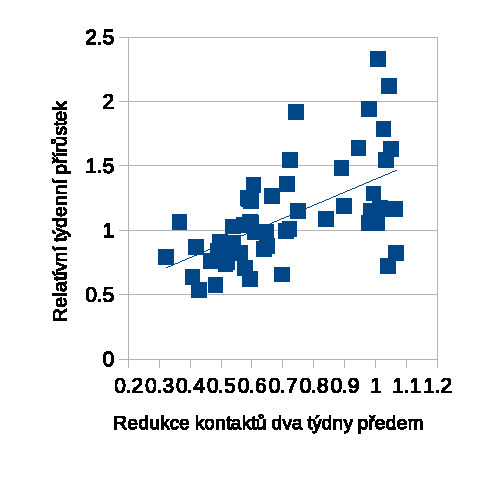
\includegraphics[scale=0.5]{pic/correl}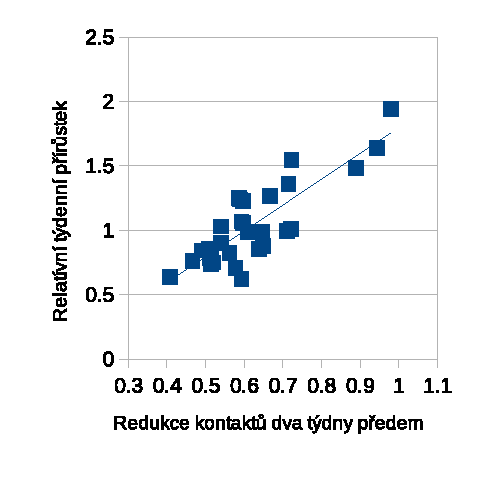
\includegraphics[scale=0.5]{pic/correl2}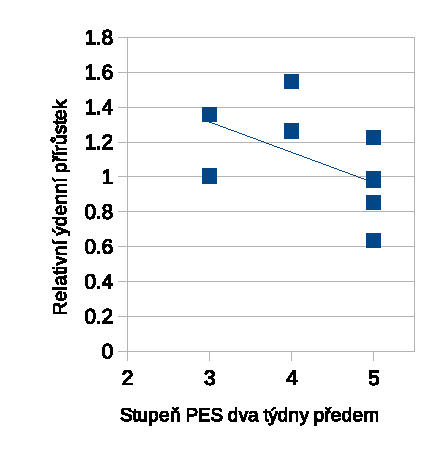
\includegraphics[scale=0.5]{pic/corpes}
\caption{Souvislost redukce kontaktů a relativního týdenního přírůstku hlášených nakažených od 23. března 2020 do 26. dubna 2021 (vlevo) a od 28. září 2020 do 26. dubna 2021 (uprostřed), souvislost stupně protiepidemického systému PES a relativního přírůstku nakažených od 23. listopadu 2020 do 25. ledna 2021 (doba fungování PES, vpravo).}
\label{fig:souvislosti}
\end{center}
\end{figure}\\
Základní statistická analýza přesvědčivě ukazuje souvislost redukce kontaktů s~nárůstem epidemie. Na levém grafu obrázku \ref{fig:souvislosti} jsou vykresleny relativní týdenní přírůstky nových
případů oproti koeficientu redukce
kontaktů, mě\-ře\-né\-mu longitudinálním sociologickým výzumem \cite{paqcovid} dva tý\-dny pře\-dem. 
Koeficient redukce nabývá hodnoty 1 v~případě,
že je množství kontaktů shodné s~dobou těsně před pandemií, a byl
by hypoteticky nulový, pokud by lidé neměli žádné rizikové kontakty.
Prostřední graf zobrazuje tytéž veličiny za kratší období počínající
28. zářím -- na rozdíl od předešlého tento graf nezobrazuje hodnoty
z~léta 2020, kdy docházelo k~lokálním vzplanutím a opatření
byla aplikována jen v~ohniscích, takže nemohla být globálním
sociologickým výzkumem reflektována. Na pravém grafu jsou zobrazeny týdenní přírůstky
nakažených oproti stupni protiepidemického
systému PES \cite{PES} dva týdny předem. \\
Spearmanův korelační koeficient
vychází u~levého grafu $0,6$ (signifikantní na $1\%$ hladině), což svědčí pro
signifikantní efekt příčin $K$, u~pravého grafu je pak Spearmanův koeficient $-0,7$1 (signifikantní na $5$\% hladině), což naopak svědčí pro $C$, byť zde jde kvůli nedostatku dat a nejasné specifikaci stupňů PES spíše o~ilustraci než solidní statistickou evidenci. Efekt $J$ (jednotlivá opatření)
by vyžadoval podrobnější analýzu, obecně je ale velice obtížné rozlišit efekty
jednotlivých opatření. Například v~práci \cite{Brauner_etal2020},
která se o~to pokouší na základě dat z~41 zemí, autoři sami přiznávají,
že jejich studie nedokáže rozlišit efekt opatření od nepřímých efektů,
jako je zvýšená opatrnost obyvatelstva. Podobné těžkosti se týkají
i vyhodnocování efektu osobní ochrany (R), nicméně zde existuje mnoho
studií měřících jejich efekt ve specifických podmínkách, například \cite{chu2020physical}.
\item \emph{Konzistence/reprodukovatelnost: efekt se vyskytuje opakovaně,
u~různých osob a v~různých prostředích (mělo by existovat více studií,
pokud možno z~různých zemí či subpopulací).}\\
Existuje dlouhá řada prací zabývajících se 
účinností nefarmaceutických intervencí, viz například \cite{flaxman2020estimating},
viz též shrnutí \cite{kluveitOpat}. 
Opakovatelnost ve smyslu simultánního výskytu v~různých geografických jednotkách podporují i data z~České republiky. Graf \ref{fig:okresy} znázorňuje závislost zjednodušeného reprodukčního čísla $R$ měřeného v~jednotlivých okresech na počtu rizikových kontaktů hlášených deset dní předem respondenty výzkumu \cite{paqcovid} žijícími v~příslušném okrese. Lineární smíšený model potvrzuje lineární závislost $R$ na počtu kontaktů jak v~období říjen-prosinec 2020, tak v~období leden--březen 2021, avšak potvrzuje také „změnu pravidel“ (zvýšení koeficientu závislosti) mezi těmito dvěma obdobími. Kromě signifikantní závislosti v~obou obdobích\footnote{Obecný lineární smíšený model s~fixními efekty a $AR(1)$ rezidui potvrzuje rostoucí závislost jak pro období říjen--prosinec 2020 ($p=0.002$, nárůst $0.00712$ na jeden dodatečný kontakt v~průměru, $CI_{0.95}=(0.0027,0.0115)$), tak pro období leden--březen 2021 ($p<0.001$, nárůst $0.0145$ na jeden kontakt v~průměru navíc na osobu, $CI_{0.95}=(0.0106,0.0184)$).} je statisticky signifikantní i rozdíl na\-kaž\-li\-vos\-ti mezi oběma obdobími,\footnote{Změna regresního koeficientu kvantifikujícího riziko kontaktů je signifikantní s~$p=0.013$.} který lze přirozeně vysvětlit nástupem nové varianty viru začátkem roku 2021 (viz též kapitolu \ref{Nekolik_poznamek}).


\begin{figure}
\begin{center}
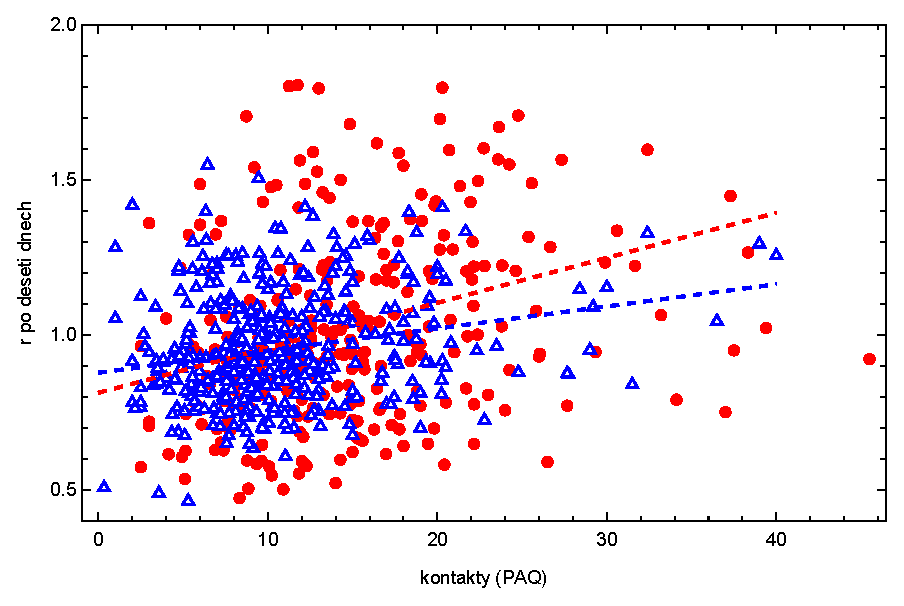
\includegraphics[width=8cm]{pic/sbornikRegrese010.eps}
\caption{Závislost zjednodušeného reprodukčního čísla na počtu rizikových kontaktů v~okresech. Modrá: říjen--prosinec 2020, červená: leden--březen 2021.}
\label{fig:okresy}
\end{center}
\end{figure}

\item \emph{Specificita: čím více lze vyloučit ostatní faktory vzniku, tím
spíš půjde o~kauzalitu.}\\
Vzhledem k~tomu, že epidemie probíhá takříkajíc za plného provozu,
to jest v~kontextu všech komplexních vlivů, kterým je člověk ve společnosti
vystaven, je potvrzení kauzality tímto způsobem velice obtížné.
Může se sice stát, že nemoc propukne v~izolovaném prostředí, jako
například na lodi Diamond Princess \cite{mizumoto2020transmission},
není nám však znám podobný případ, který by přinesl výsledky týkající
se účinnosti protiepidemických opatření. 
\item \emph{Časovost: následek musí nastat později než příčina (člověk musí
nejdříve mít rizikové kontakty, pak onemocnět).}\\
Vzhledem k~současným pokročilým metodám sběru dat a jejich ukládání
jsou, zejména ve vyspělejších státech, k~dispozici poměrně přesné
časové údaje o~vý\-vo\-ji počtu hlášených případů, což dovoluje i zkoumání časovosti.
V~případě tý\-den\-ních dat z~České republiky nejlepší shodu, měřenou
korelačním koeficientem, dává dvoutýdenní až třítýdenní zpoždění mezi měřením
kon\-tak\-tů a hlášením pří\-růst\-ku, viz obrázek \ref{fig:korelace}.
\begin{figure}
\begin{center}
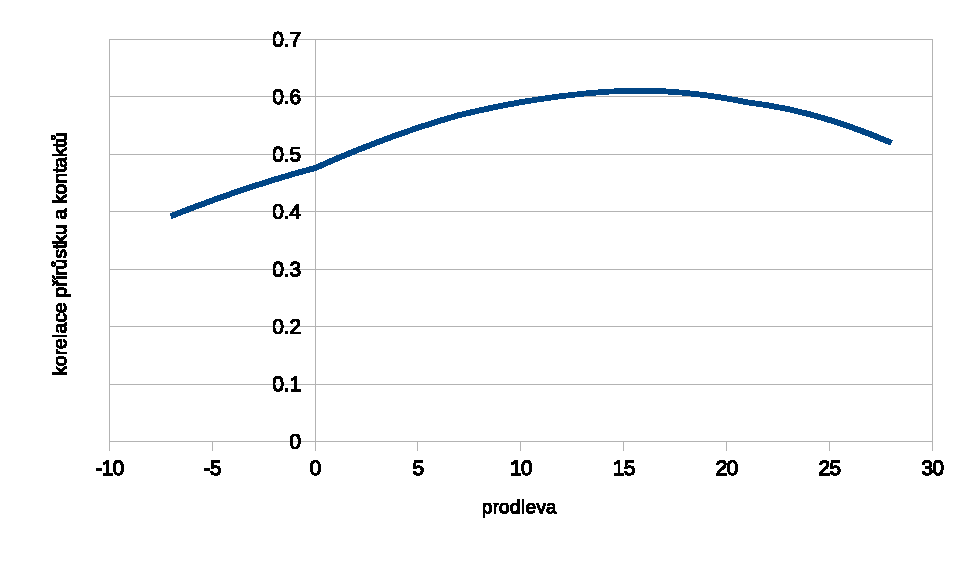
\includegraphics[width=8cm]{pic/lagsel.eps}
\caption{Korelace hlášených případů a počtu rizikových kontaktů pro různá zpoždění.}
\label{fig:korelace}
\end{center}
\end{figure}
\item \emph{Biologický gradient: větší expozice vzhledem k~příčině znamená
větší efekt (větší počet kontaktů znamená větší pravděpodobnost nakažení,
častější nošení roušky menší pravděpodobnost atd.).}\\
V~komentáři k~prvnímu kritériu (síla efektu) jsme konstatovali, že závislost přírůstku infekcí a redukce kontaktů je statisticky signifikantní. To však samo o~sobě neimplikuje existenci biologického gradientu -- (Spearmanova) korelace by mohla vyjít signifikantní například i v~případě, že by po určitou hodnotu redukce byly přírůstky stejné a pak teprve začaly růst. Jak ale naznačuje obrázek \ref{fig:souvislosti} uprostřed, nic takového se neděje: přírůstky případů s~hodnotou redukce vždy rostou, z~čehož vyplývá i existence
biologického gradientu, jejich závislost se navíc jeví lineární, což umožňuje gradient jednoduše kvantifikovat.
\item \emph{Plausibilita: Je vhodné (ne však nutné) znát mechanismus způsobující
efekt.} \\
Tato podmínka je zde splněna takříkajíc triviálně, neboť je známo,
že k~přenosu dochází téměř výhradně prostřednictvím kontaktů mezi lidmi
(což vysvětluje $K$) prostřednictvím kapének či aerosolů (což vysvětluje
$R$, viz též kapitolu \ref{Co_se_vi}) -- zprostředkovaně je tak vysvětleno i $C$, případně $J$.
\item \emph{Koherence: Je vhodné (ne však nutné), aby zkoumaný vztah odpovídal
laboratorním zjištěním.}\\
Současný rozsáhlý laboratorní výzkum SARS-CoV-2 přinejmenším neodporuje
hypotéze účinnosti používaných nefarmaceutických opatření, naopak
je často podporuje. Změna nakažlivosti, zmiňovaná u~druhého kritéria, například dobře odpovídá údajům o~rostoucí prevalenci nakažlivější mutace B.1.1.7 (viz například \cite{diana}).
\item \emph{Experiment: Je vhodné (pokud je to možné), aby byl daný vztah
prokázán experimentální evidencí.}\\
Je jasné, že laboratorní experimenty pro potvrzení účinnosti protiepidemických
opatření nelze z~etických důvodů pořádat. Někdy se takový experiment \uv{po\-da\-ří} uspo\-řá\-dat v zemi, kde jsou vyžadovány nižší etické standardy \cite{abaluck2021impact}, může se však vyskytnout i příležitost s etikou nekolidující:
takzvaný přirozený experiment -- jeden z~těchto případů, mimo jiné potvrzujících
roli rizikových kontaktů v~šíření SARS-CoV-2, je popsán v~kapitole
\ref{Prirozene_experimenty}.
\item \emph{Analogie: Někteří autoři považují za vhodné, pokud jsou 
uvedeny přesvědčivé analogie či podobnost s~jinými jevy.}\\
Zdá se více než pravděpodobné, že relativně lepší zvládnutí pandemie
vý\-cho\-do\-asij\-ský\-mi státy souvisí s~jejich poměrně čerstvou zkušeností
s~nákazou SARS, zatímco v~Evropě a USA byla poslední 
výzvou podobného rozsahu pandemie španělské chřipky před sto lety. Je velmi těžké odhadnout,
jak by byla pandemie celosvětově zvládnuta, nebýt těchto čerstvých
asijských zkušeností.
\item \emph{Reverzibilita: Pokud příčina zmizí, zmizí efekt.}\\
Podobně jako v~případě experimentů potvrzení kauzality tímto způsobem
na\-rá\-ží na etické limity, například zrušení protiepidemických opatření kvůli experimentu není z~etických důvodů možné. Během více než roku trvání pandemie tato situace přesto ve světě několikrát nastala, většinou z~důvodů neochoty politické
reprezentace k~zavedení protiepidemických opatření. Ikonický je
v~tomto směru případ brazilského velkoměsta Manaus, kde se virus na
jaře 2020 rozšířil do té míry, že se usuzovalo, že bylo dosaženo kolektivní
imunity. Navzdory tomuto přesvědčení se však v~lednu ve městě objevila
nová vlna onemocnění \cite{sabino2021resurgence}. 
Případ Manaus je pro naši diskusi velice důležitý, neboť jako jeden z~mála
prolomil takzvaný paradox prevence, spočívající v~tom, že jev, před kterým prevence chrání, díky prevenci nenastane, což slouží odpůrcům prevence jako argument proti této prevenci. Právě v~Manaus se ukázalo, k~jakým následkům absence nefarmaceutických opatření vede.

\end{enumerate}

Shrnutí: Pokud chceme usuzovat na nějakou kauzalitu, je dobré mít ji takříkajíc potvrzenou z~více zdrojů. Jinými slovy: Naše hypotéza by měla být konzistentní s~ostatními vědeckými zjištěními. Užitečnou pomůckou k~identifikaci kauzality v~epidemiologii jsou Hillova kritéria, která jsme demonstrovali na příkladu vztahu růstu epidemie a nefarmaceutických opatření. Jelikož naše hypotéza o~účinnosti zmíněných opatření „sítem“ těchto kritérií poměrně úspěšně prošla, vyslovili jsme pádný argument v~diskusi o~účinnosti předložených opatření.

\subsection*{Diskuse}

Jak už jsme uvedli výše, naším cílem nebylo přinést nějaké převratné
vhledy do problematiky kauzality v~epidemiologii, ostatně to, co zde
„dokazujeme“, je spíše trivialita, o~které se v~solidních vědeckých
kruzích patrně vůbec nediskutuje. I~přístup, který jsme použili, je
spíše učebnicový -- za více než padesát let od Hillova článku se
diskuse na dané téma značně posunula, viz například \cite{rothman2005causation}.
Naším hlavním cílem bylo naznačit možný způsob „rozsouzení“ různých kontroverzí týkajících se (nejen) současné epidemie. 

V~těchto kontroverzích však zdaleka nezaujímáme neutrální pozici. Z~našeho, byť triviálního, příkladu je jasné, jak hluboce je takzvaný hlavní proud ve srovnání s~různými „disentními“
názory zakotven ve vědeckém uvažování a jak nesrovnatelně lépe je
odůvodněn. Naopak, pokud například \cite{wood2021inferring} naznačuje, že fatální infekce
začaly klesat ještě před zavedením britského lockdownu, je k~této
myšlence nutno i přes všechnu statistickou sofistikovanost práce přistupovat
s~krajní o\-be\-zřet\-nos\-tí, protože tvrzení, implicitně z~této domněnky
vyplývající, totiž že epidemie se v~raných fázích svou vnitřní dynamikou
sama utlumí, nemá kromě uvedené statistické evidence (tedy první podmínky) podporu v~žádném dalším bodu Hillova seznamu. Podobně pokud \cite{KomarekStraka2021} tvrdí, že většina opatření neměla významný vliv na dynamiku epidemie, a dokládají to údajně chybějícími časovými souvislostmi svého odhadu reprodukčního čísla a opatření, přinejmenším dluží vysvětlení, co v~tom případě vliv mělo, včetně pečlivého odůvodnění, třeba pomocí Hillova seznamu, že jde skutečně o~kauzalitu.
